\section{SpECTRE Elliptic Solver}

\subsection{Overview}
\frame{
\frametitle{SpECTRE Elliptic Solver}
\begin{center}
      
\includegraphics[width=.8\textwidth]{pictures/spectrells.pdf}\\
  \begin{block}{\centering Components}
\begin{itemize}
\scriptsize
\item[\blacksquare]PDE Discretization: \textbf{Discontinuous Galerkin}
\item[\blacksquare]Adaptive Mesh Refinement: \textbf{hp-AMR}
\item[\blacksquare]Parallel Mesh Storage  \textbf{Parallel Forest of Octrees}
\item[\blacksquare]Linear system solver: \textbf{Multigrid Preconditioner + PETSc Iterative solver}
\item[\blacksquare]Visualization: \textbf{yt}
\end{itemize}   
  \end{block}
\end{center}
}

\subsection{Discontinuous Galerkin}
\frame{
  \frametitle{Traditional Discretization Schemes}

{\scriptsize
Finite difference and Spectral Finite Elements are currently used.
We write the PDE as

\begin{equation*}
\label{eq:1}
\begin{split}
&R(u) = 0 \\
\rightarrow &R_{h}(u) \approx 0 \text{    (on a computer)}
\end{split}
\end{equation*}
}
  \begin{columns}
    \begin{column}{.48\textwidth}
% First formulated in 1970, dG methods were largely ignored until recently.
% \vspace{1cm} 
%       \begin{block}{Advantages of dG}
%         \begin{enumerate}
%         \item[\blacksquare]hp-adaptive
%         \item[\blacksquare]easily parallelized
%         \item[\blacksquare]conceptually similar in n-d
%         \item[\blacksquare]small local operators
%         \item[\blacksquare]different numerical fluxes
%         \end{enumerate}
      % \end{block}
\begin{mybox}{white}{\centering Finite Difference}
% \centering \scriptsize \underline {Finite Difference}\\
\scriptsize
\begin{itemize}
\item[\blacksquare]Simple to code 
\item[\blacksquare]Algebraically convergent
\end{itemize}
      \begin{center} 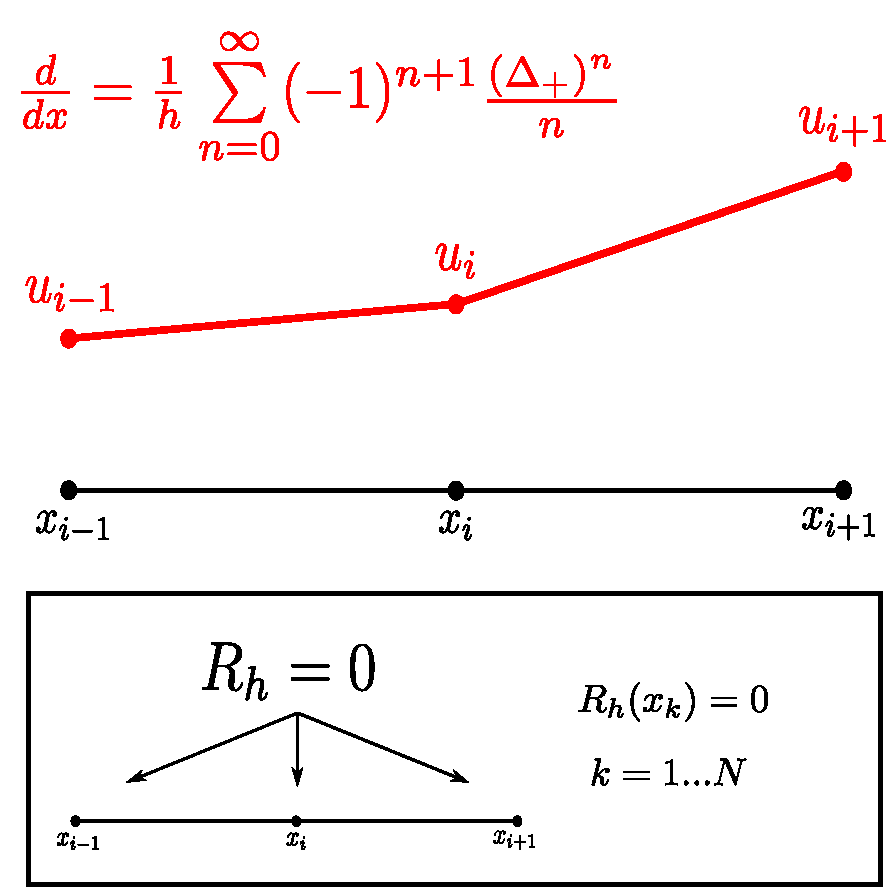
\includegraphics[width=.85\textwidth]{pictures/fd.pdf}\\
\end{center}
\end{tcolorbox}
    \end{column}
    \begin{column}{.48\textwidth}
\begin{mybox}{white}{\centering Spectral FEM}
% \centering \scriptsize  \underline {Spectral FEM}\\
\scriptsize
\begin{itemize}
\item[\blacksquare]Hard to code 
\item[\blacksquare]Exponentially convergent
\end{itemize}
      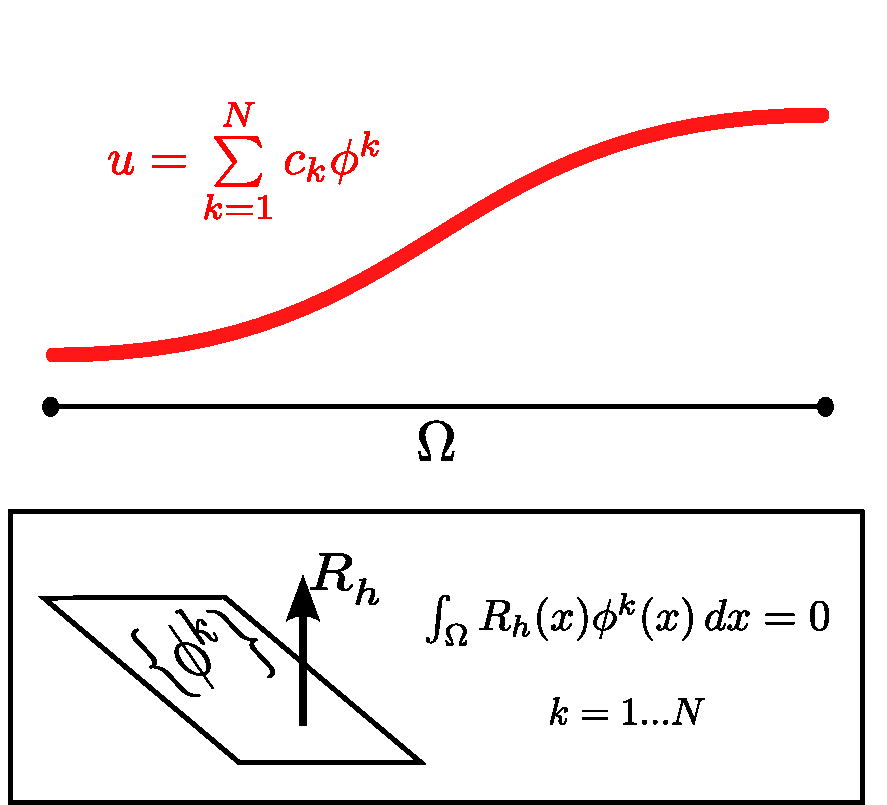
\includegraphics[width=\textwidth]{pictures/spectral.pdf}      
\end{mybox}
    \end{column}
  \end{columns}

}

\frame{
  \frametitle{Discontinuous Galerkin (DG)}

  \begin{columns}
    \begin{column}{.48\textwidth}
$\,\,$\\
\vspace{.5cm}
First used in 1970 by \\ Reed and Hill. \\ 
\vspace{.2cm}
DG methods were largely ignored until recently.\\
\vspace{.3cm} 
\begin{mybox}{white}{\centering Discontinuous Galerkin}
      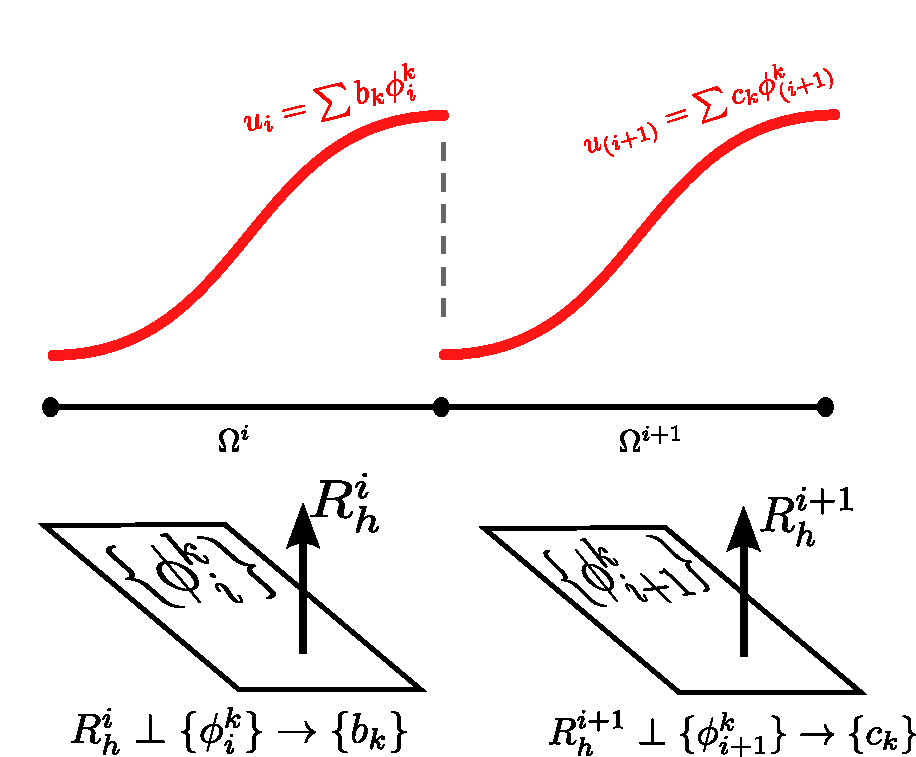
\includegraphics[width=\textwidth]{pictures/dg2.pdf}      \\
\end{mybox}
    \end{column}
    \begin{column}{.48\textwidth}
      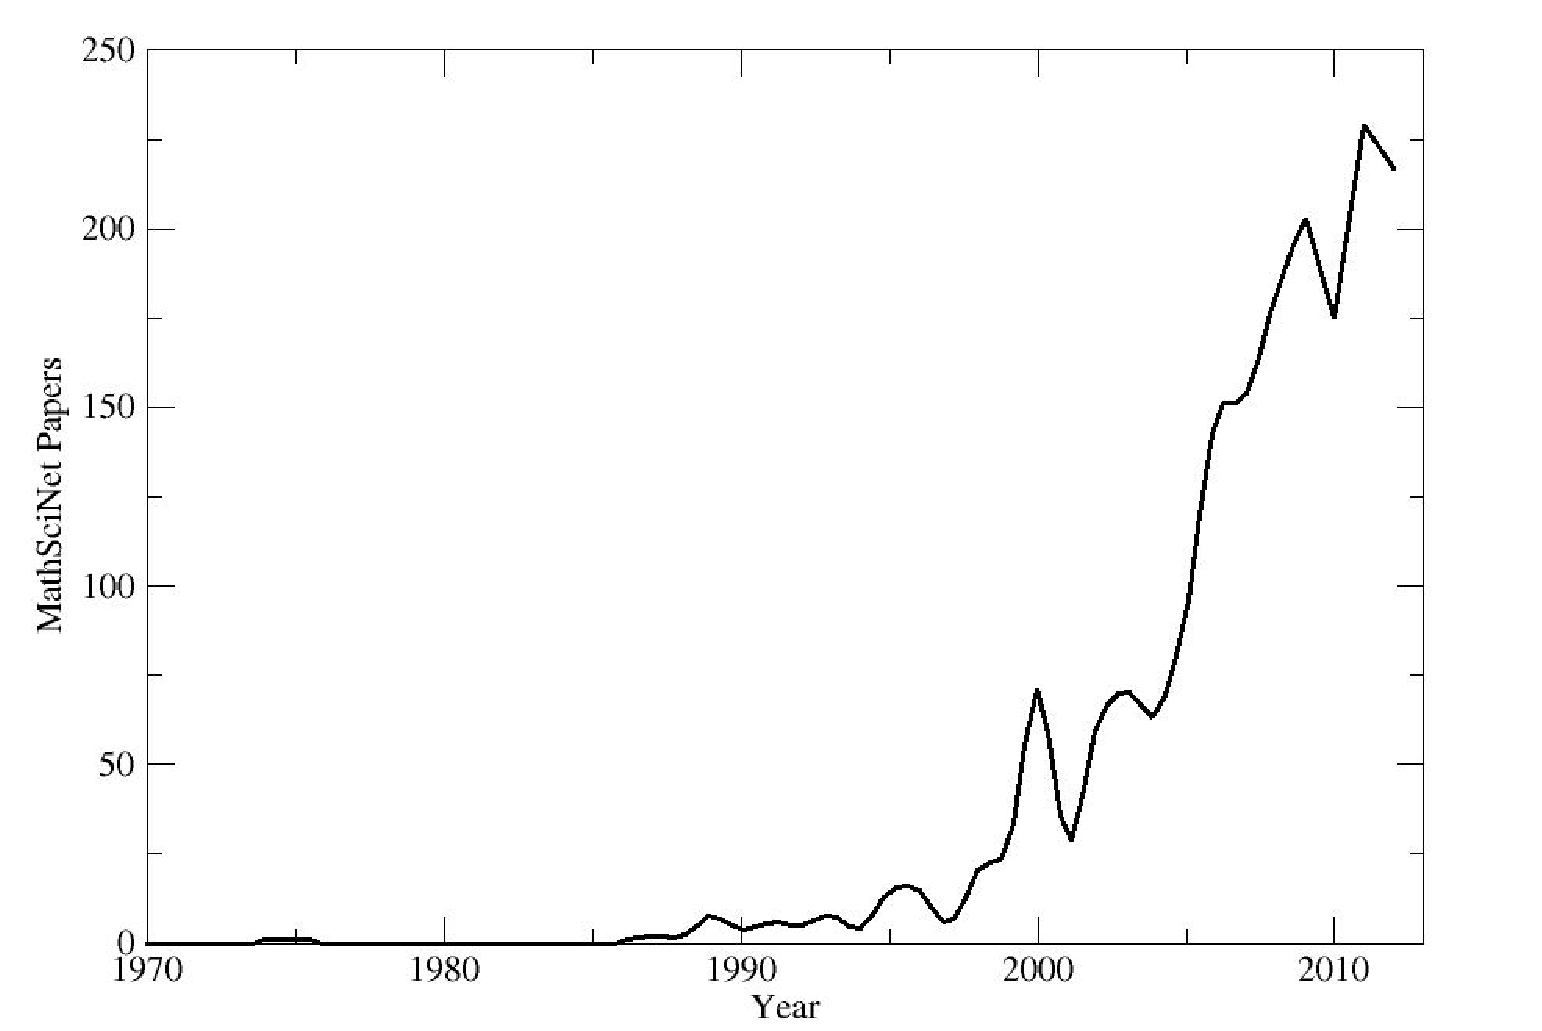
\includegraphics[width=\textwidth]{pictures/dg.pdf}\\
\vspace{-.2cm}
\centering {\tiny  [Di Pietro, Ern; Springer 2012]}
      \begin{block}{\centering Advantages of dG}
        \begin{enumerate}
        \item[\blacksquare]hp-adaptive
        \item[\blacksquare]easily parallelized
        \item[\blacksquare]conceptually similar in n-d
        \item[\blacksquare]small local operators
        \end{enumerate}
      \end{block}
    \end{column}
  \end{columns}

}

\subsection{hp-AMR}
\begin{frame}
\frametitle{Adaptive Mesh Refinement}
\begin{columns}
  \begin{column}{.6\textwidth}
% \begin{itemize}
% \item[\blacksquare]BNS length scales:
\begin{center}
\vspace{.5cm}
\setul{}{2pt}
\ul{NSNS Coalescence Length Scales}
\vspace{.3cm}
  \begin{enumerate}
  \item[\blacksquare] internal NS dynamics\footnote[frame]{\scriptsize Assuming Polytropic EOS} $\approx 0.1M_{NS}$ 
  \item[\blacksquare] evolution time scale $\approx 0.1M_{NS}$
  \item[\blacksquare] orbital separation $\approx 50M_{NS}$
  \item[\blacksquare] wave zone boundary $\approx 1000M_{NS}$
  \end{enumerate} 
\end{center}
\vspace{1cm}
  \end{column}
  \begin{column}{.35\textwidth} 
\begin{center}
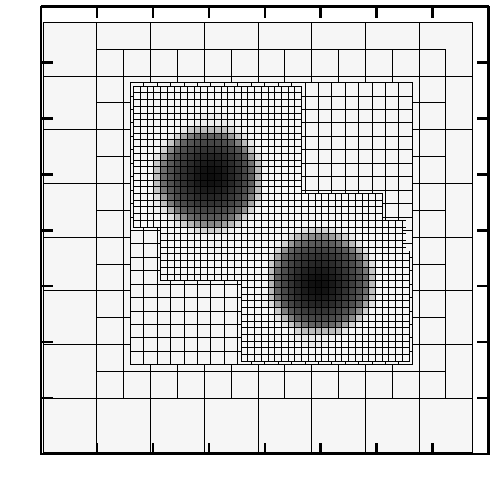
\includegraphics[width=\textwidth]{pictures/ns_amr.pdf}
\vspace{-.15cm}   
\text{ \scriptsize [Evans et al; gr-qc/0501066]}
\end{center}
% \vspace{.5cm}
    % \includegraphics[width=\textwidth, height=.7\textwidth]{pictures/nbody_wakes_cropped.pdf}
  \end{column}
\end{columns}

\end{frame}

\frame{
\frametitle{hp-Adaptive Mesh Refinement}

\begin{mybox}{white}{}
\centering {dG naturally allows for hp-adaptivity}\\
\end{mybox}
\vspace{.1cm}

\begin{columns}
  \begin{column}{.48\textwidth}
\centering
% \begin{itemize}
% \item[\blacksquare]BNS length scales:
\begin{itemize}
\item[\blacksquare] \textbf{h-refinement} for discontinuous regions \\
\vspace{.75cm}
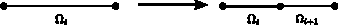
\includegraphics[width=.8\textwidth]{pictures/hrefine.pdf} \\
 \end{itemize}
\vspace{.5cm}
\centering 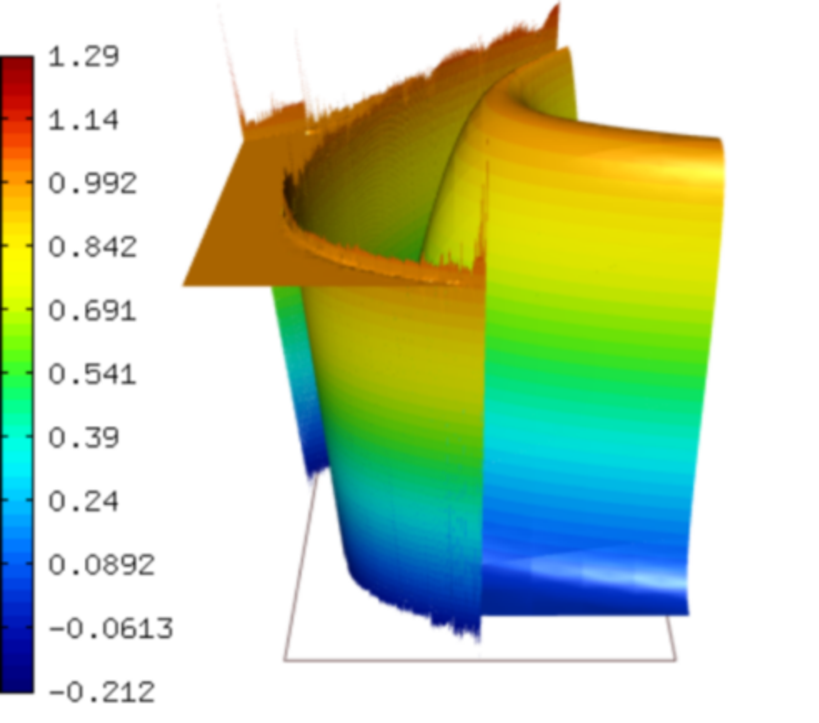
\includegraphics[width=.7\textwidth]{pictures/hermes1.pdf} \\


% \end{itemize}    
  \end{column}
  \begin{column}{.48\textwidth} 
\begin{center}
% \tiny{advection-reaction problem with hp-AMR}
 % 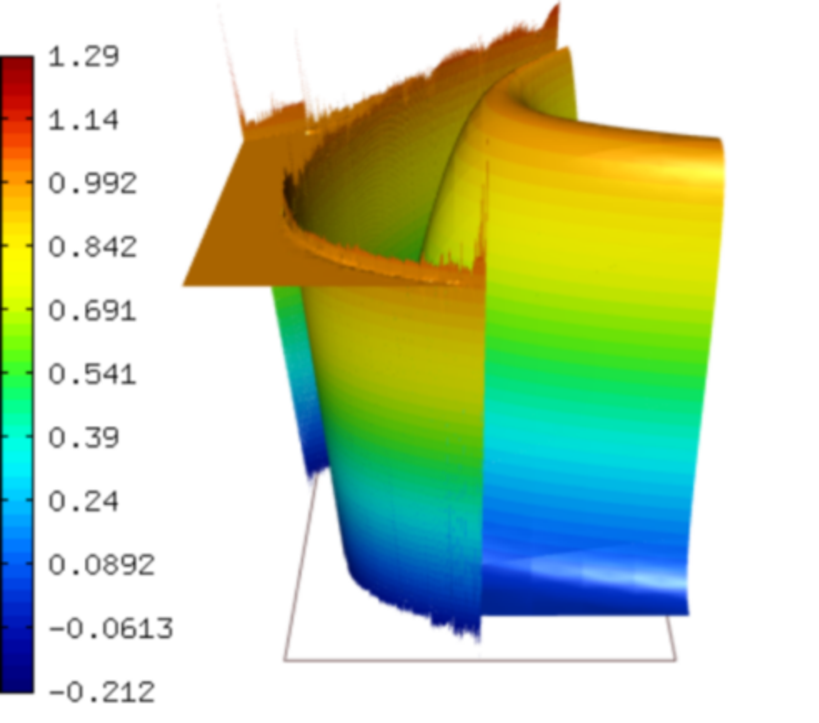
\includegraphics[width=\textwidth]{pictures/hermes1.pdf} \\   
\vspace{-.4cm}
\begin{itemize}
 \item[\blacksquare]\textbf{p-enrichment} for smooth regions \\
\vspace{.65cm}
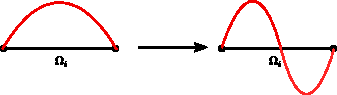
\includegraphics[width=.8\textwidth]{pictures/prefine.pdf} \\
\end{itemize}
\vspace{.3cm}
 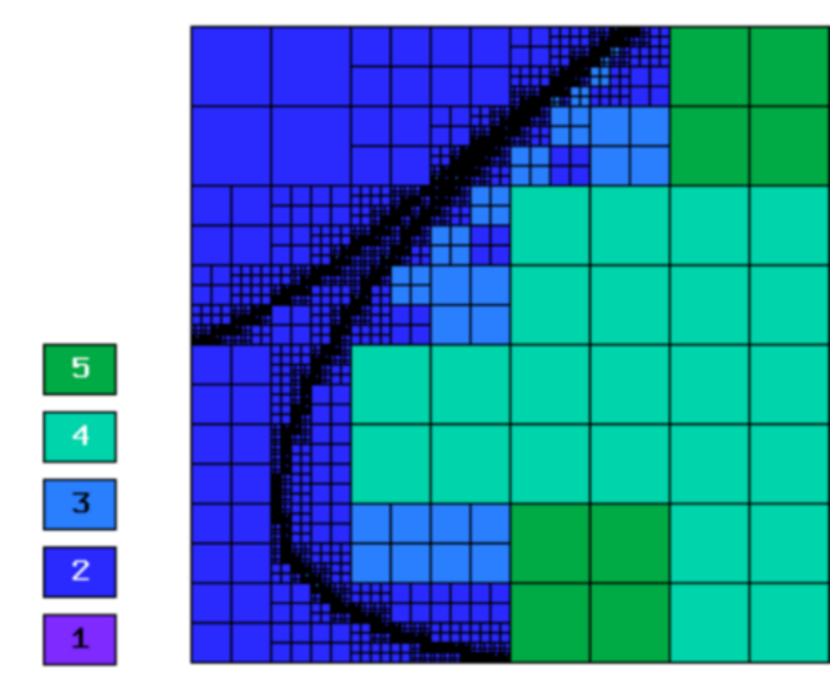
\includegraphics[width=.6\textwidth]{pictures/hermes2.pdf} \\
\end{center}
% \vspace{.5cm}
    % \includegraphics[width=\textwidth, height=.7\textwidth]{pictures/nbody_wakes_cropped.pdf}
  \end{column}
\end{columns}
\vspace{.2cm}   
\centering \text{ \scriptsize [hpfem.com/hermes]}
  % discontinuous Galerkin naturally allows for hp-AMR
}

\subsection{Forest of Octrees}
\frame{
\frametitle{p4est: Parallel AMR on a Forest of Octrees}
    \begin{itemize}
    \item[\blacksquare]distributed octrees for PDE meshes
    \item[\blacksquare]load balancing
    \item[\blacksquare]scale-tested on $O(500k)$ cores
    \end{itemize}
\begin{columns}
  \begin{column}{.48\textwidth}

    \begin{center}
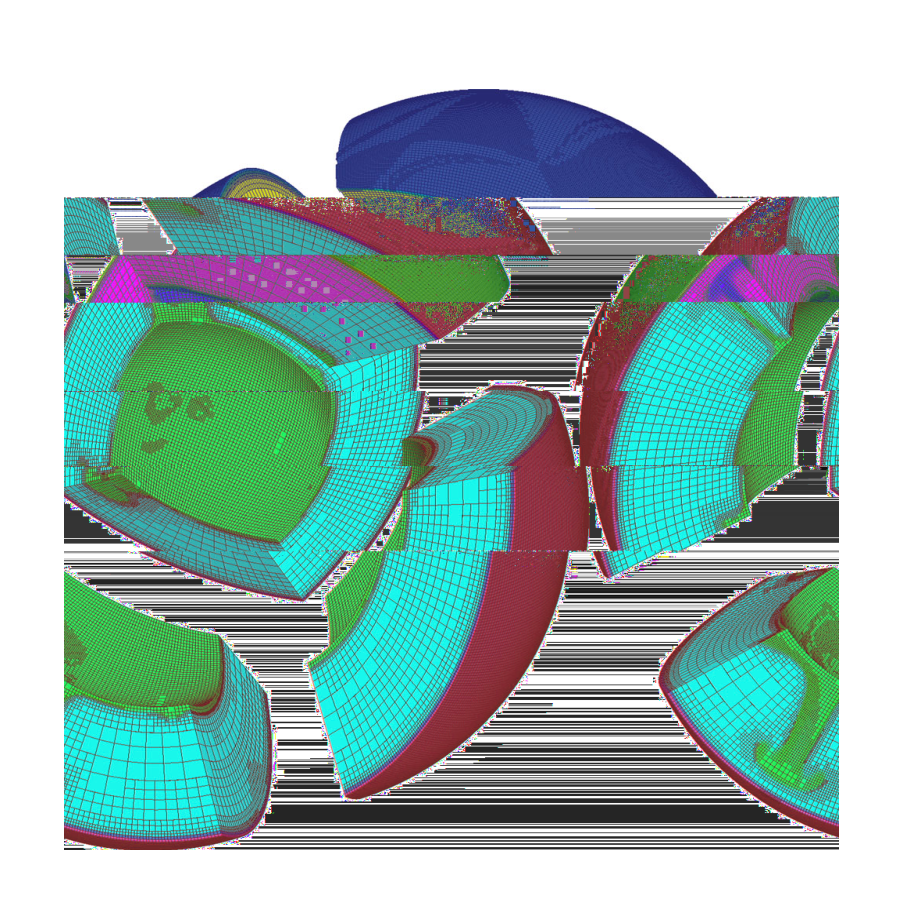
\includegraphics[width=\textwidth]{pictures/earthmantle_cropped.pdf}\\
\vspace{-.4cm}  
{\tiny Mantle simulation with 24-octrees.}      
    \end{center}

  \end{column}
\begin{column}{.4\textwidth} 
    \begin{center}
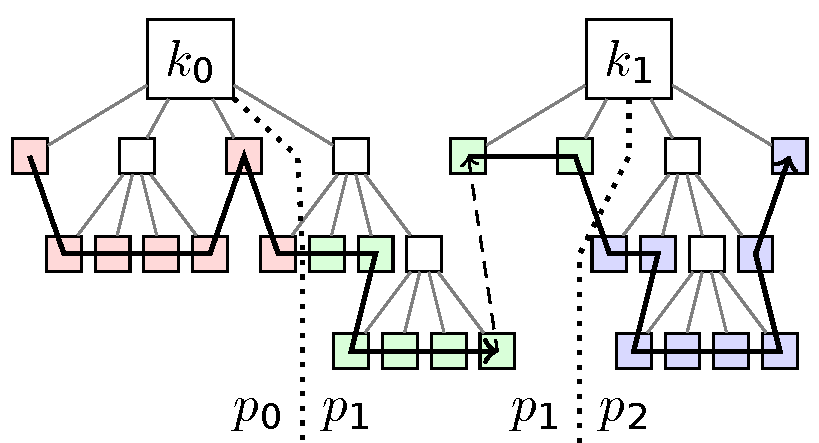
\includegraphics[width=\textwidth]{pictures/p4esttrees_cropped.pdf}\\
% 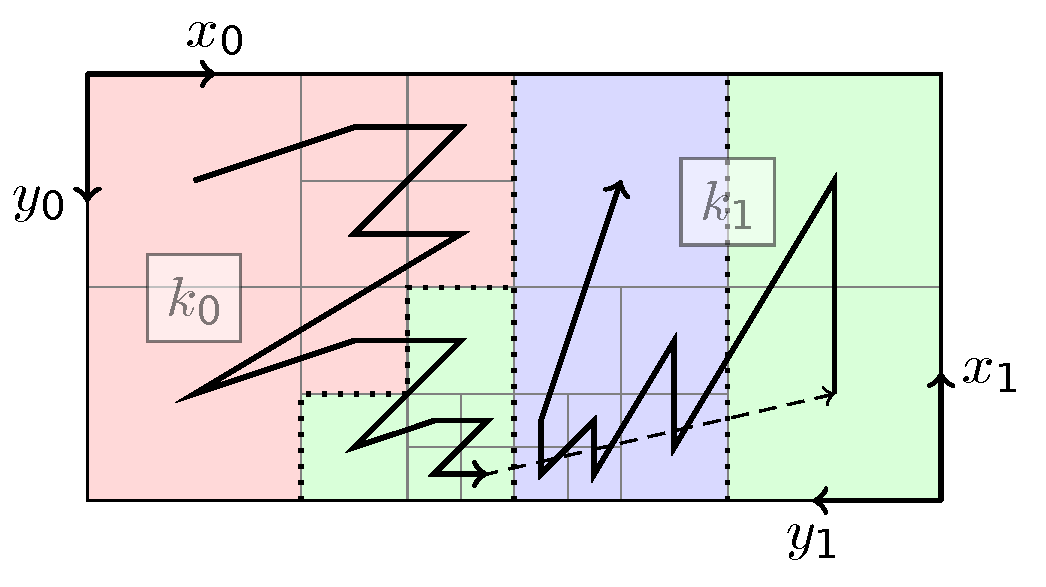
\includegraphics[width=\textwidth]{pictures/p4estblocks_cropped.pdf}\\
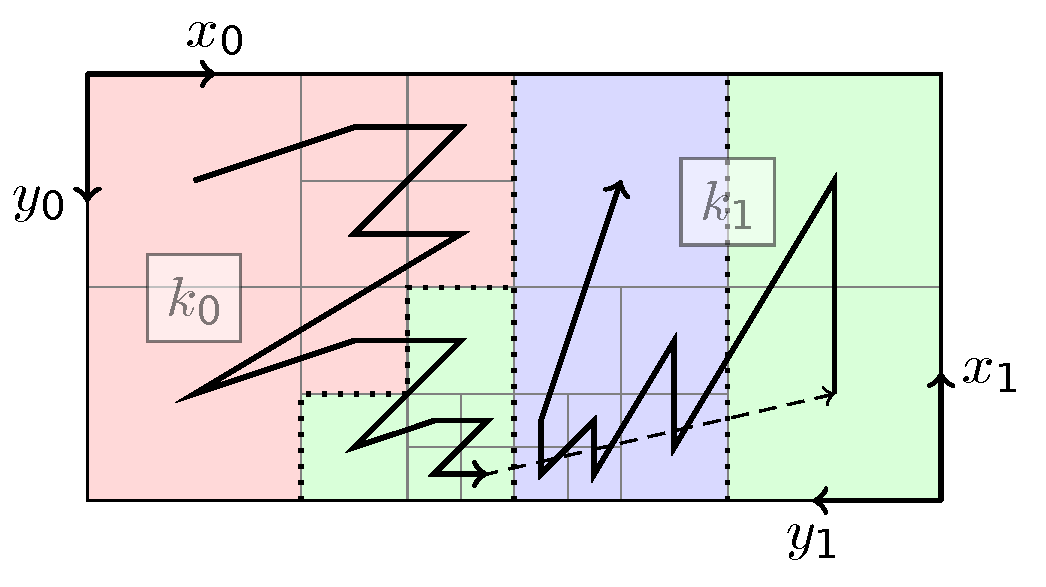
\includegraphics[width=\textwidth]{pictures/p4estblocks_cropped.pdf}
\vspace{-.3cm}  
{ \tiny [Burstedde et al; 1406.0089]}
   \end{center}
\end{column}
\end{columns}

}

% \begin{frame}
% \frametitle{p4est: Scaling Example}
% \label{sec-2-2}
% \begin{columns}
% \begin{column}{.4\textwidth}
% %% Column 1
% \label{sec-2-2-1}

% \tiny Sundar, Hari, et al. ``Parallel geometric-algebraic multigrid on unstructured forests of octrees.'' Proceedings of the International Conference on High Performance Computing, Networking, Storage and Analysis. IEEE Computer Society Press, 2012.
% \begin{block}{\small Variable Coefficient Poisson}
% \label{sec-2-2-2}

%      \vspace{-.5cm}
%      \begin{equation*}
%      \begin{split}
%      & \nabla \cdot (\mu( \vec x) \nabla u ( \vec x) ) = f(x)  \,\,\,\, \vec x \in \Omega \\
%      & u(\vec x ) = 0 \,\,\,\, \vec x \in \partial \Omega \\
%      \end{split}
%      \end{equation*}
% \centering 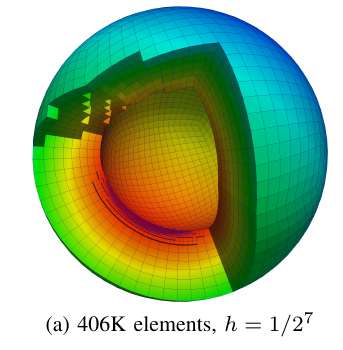
\includegraphics[width=.6\textwidth]{pictures/finegrid_gmg.png}
% \end{block}
% \end{column}
% \begin{column}{.48\textwidth}
% %% Column 1
% \label{sec-2-2-3}
% \begin{block}{\small \centering Weak Scaling}
% \label{sec-2-2-4}

% \centering 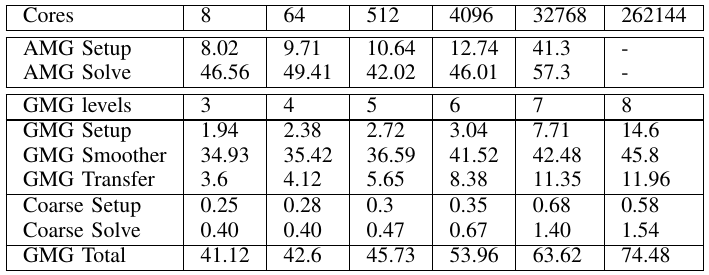
\includegraphics[width=\textwidth]{pictures/weak_scaling_sphere.png}
% \end{block}
% \begin{block}{\small \centering Strong Scaling}
% \label{sec-2-2-5}

% \centering 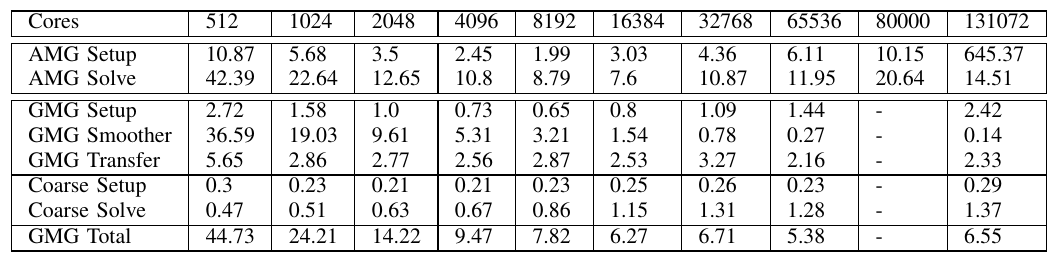
\includegraphics[width=\textwidth]{pictures/strong_scaling_sphere.png} \\
% \end{block}
% \end{column}
% \end{columns}
% \end{frame}


\subsection{Multigrid + Iterative Solver}
\label{subsec:label}
\frame{
  \frametitle{Multigrid + Krylov Iteration}

\textbf{Once discretized, elliptic PDEs boil down to:}
\begin{center}
\begin{minipage}{5cm}
\begin{block}{\centering $N \times N$ Linear System}
\centering{$Au=b$}
\end{block}
\end{minipage}
\end{center}
\scriptsize
\vspace{.5cm}
\centering{\textbf {Two Main Solution Methods}}
\begin{columns}
  \begin{column}{.55\textwidth}
    \begin{block}{\centering Direct Methods}
      % \begin{}
\centering{$u = A^{-1}b$}
      % \end{equation*}
      \begin{itemize}
      \item[\blacksquare]$O(N^{2})$ storage
      \item[\blacksquare]no pre-conditioning 
      \item[\blacksquare]ruins operator locality
      \end{itemize}

    \end{block}
  \end{column}
  \begin{column}{.4\textwidth}
% \vspace{-.92cm}
    \begin{block}{\centering Iterative Methods}
      % \begin{equation*}
        \centering{$u_k = u_{k-1} + \alpha d_{k}$}
      % \end{equation*}
\begin{itemize}
      \item[\blacksquare]$O(N)$ storage
      \item[\blacksquare]pre-conditioning
      \item[\blacksquare]preserves operator locality
\end{itemize}
    \end{block}
  \end{column}
\end{columns}

\begin{mybox}{white}{}
\centering \bf Optimal combination: Multigrid preconditioner + Iterative Solver \\
{\tiny [Wathen; 2015]}
\end{mybox}
}

% \frame{
%   \frametitle{Multigrid Preconditioner}

% {\scriptsize Preconditioning is a technique for minimizing $\kappa(A) = \frac{\lambda_{max}}{\lambda_{min}}$.}

% % \textbf{Once discretized, elliptic PDEs boil down to:}
% \vspace{-.5cm}
% \begin{center}
% \begin{minipage}{5cm}
% \begin{block}{\centering Preconditioning}
% \centering{$M^{-1}Ax=M^{-1}b$}
% $\kappa(M^{-1}A) \ll \kappa(A)$
% \end{block}
% \end{minipage}
% \end{center}

% {\scriptsize The most robust, scalable pre-conditioner known is multigrid [Wathen et al; 2015].}

% % 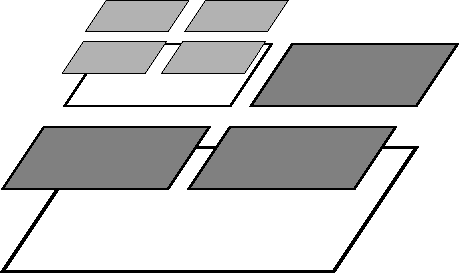
\includegraphics[width=\textwidth]{pictures/multigrid.pdf}\\
% % \begin{block}{\centering [Tatebe et al; 1994]}
% \vspace{.5cm}
%   \begin{columns}

%     \begin{column}{.4\textwidth}
% \centering{

% \begin{block}{\centering [Tatebe et al; 1994]}
% \vspace{-.3cm}
%   \begin{equation*}
%     \nabla (k \nabla u) = f \\ \\
%   \end{equation*}

%   \vspace{-2cm}
% \begin{equation*}
% \label{eq:4}
% \tiny
% \begin{split}
%  \Omega &\equiv [0,1] \times [0,1] \\
% u &\equiv 0 \,\,\, on \,\,\, \partial \Omega \\
% k &\equiv \text{discontinuous function} \\
% f &\equiv \text{discontinuous function} \\
% \end{split}
% \end{equation*}
% \end{block}
% % \normalsize
% }
%       % $- $ 
%       % $ \Omega \equiv [0,1] \times [0,1]$ \\ \\
% % $u \equiv 0$ on $\partial \Omega$\\
% % }
% % k,f are discontinuous
%     \end{column}
%     \begin{column}{.55\textwidth}
%       \centering \fbox{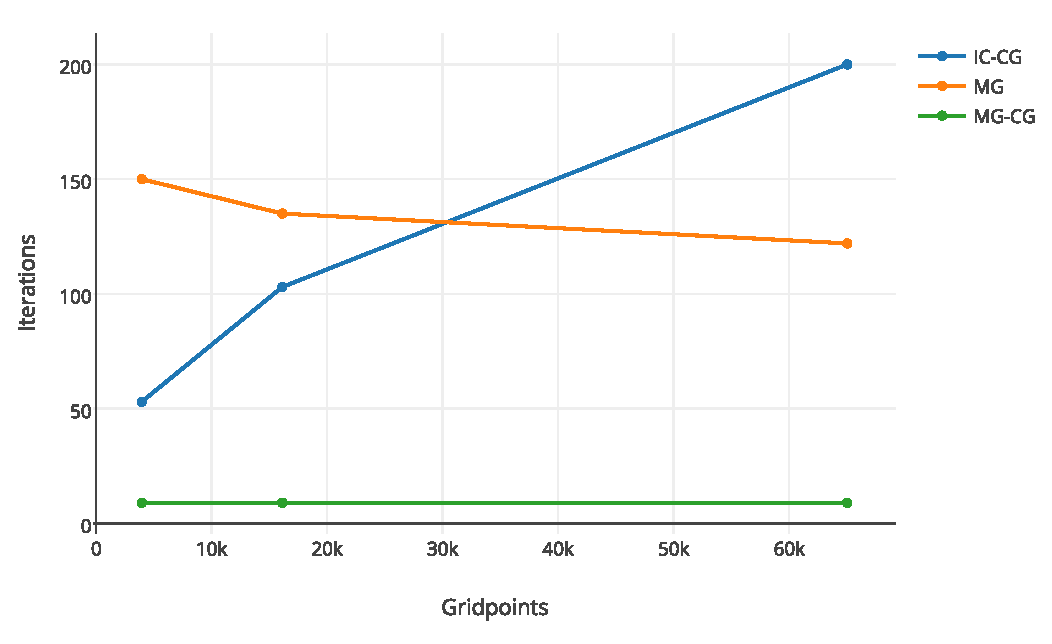
\includegraphics[width=\textwidth]{pictures/MGCG_cropped.pdf}}
%     \end{column}
%   \end{columns}
% % \end{block}
% }


\subsection{yt visualization}
\label{subsec:label}
\frame{
  \frametitle{yt visualization @ yt-project.org}
\begin{columns}
  \begin{column}{.48\textwidth}
$\,\,\,$\\
\vspace{.2cm}
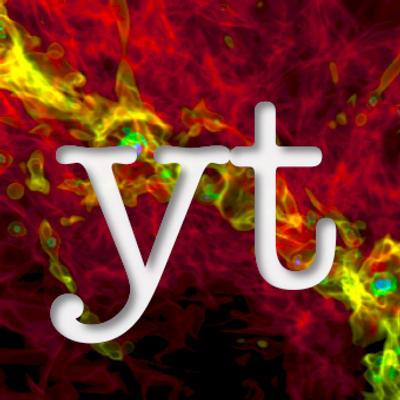
\includegraphics[scale=0.04]{pictures/ytlogo.png}
{\small \, is a python package for}
\centering
{\small visualizing volumetric, }
{\small multi-resolution data from}
{\small astrophysical simulations. } \\
\vspace{.8cm}
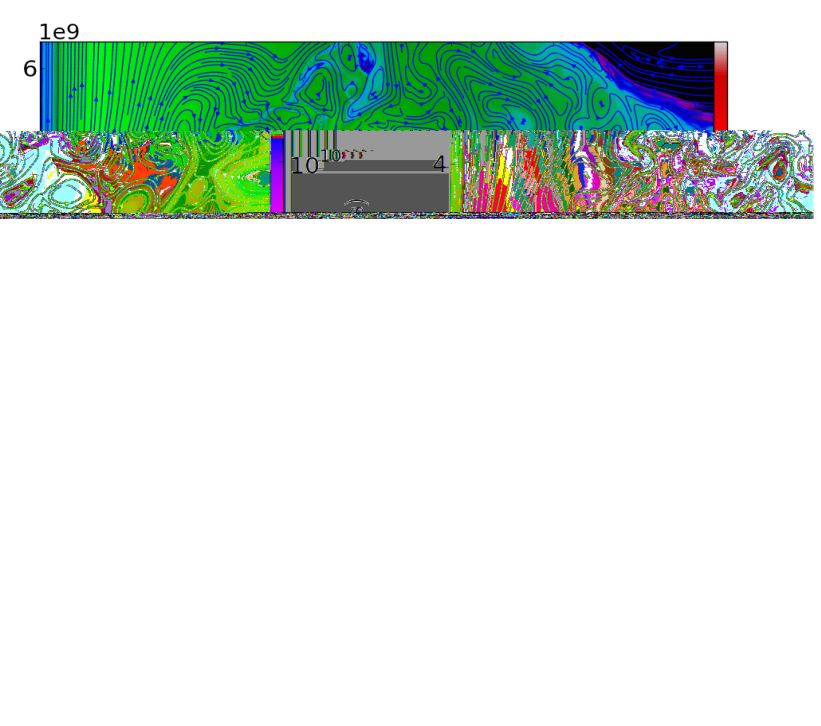
\includegraphics[width=\textwidth]{pictures/ji1_cropped.pdf}\\

  \end{column}
\begin{column}{.48\textwidth} 

% 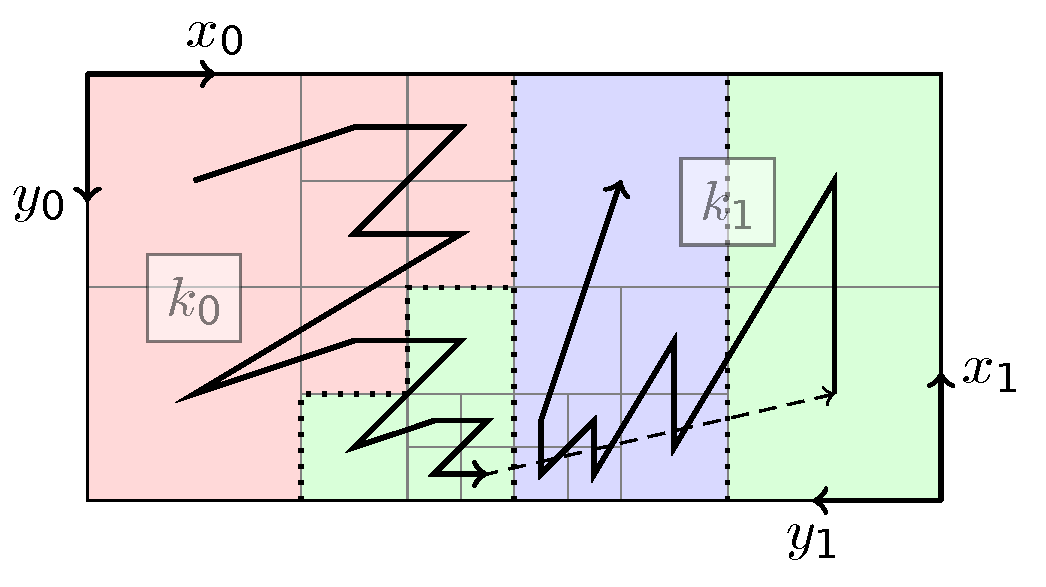
\includegraphics[width=\textwidth]{pictures/p4estblocks_cropped.pdf}\\
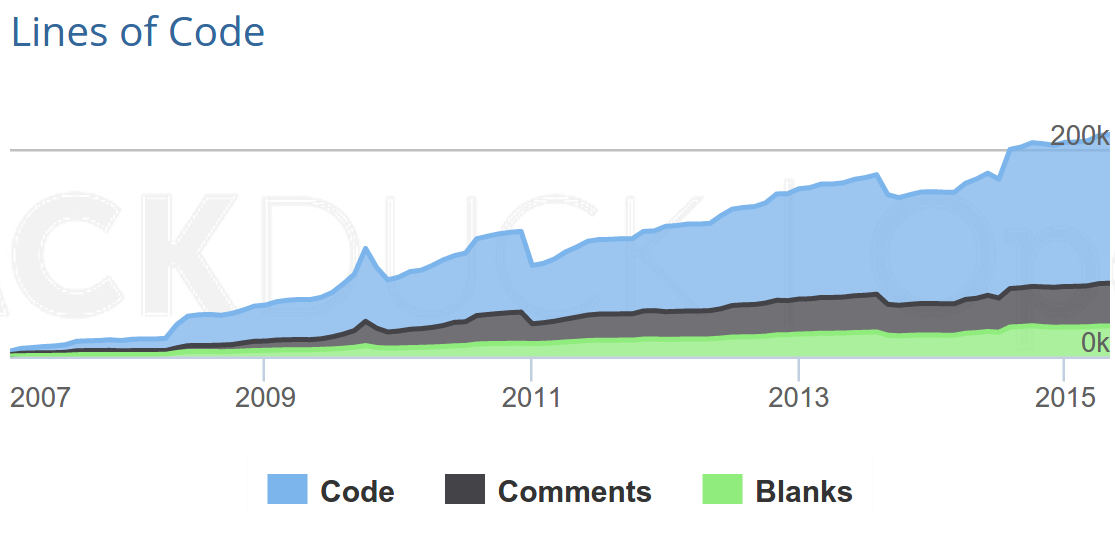
\includegraphics[width=\textwidth,height=.5\textwidth]{pictures/ytlines.png} \\
\vspace{.6cm}
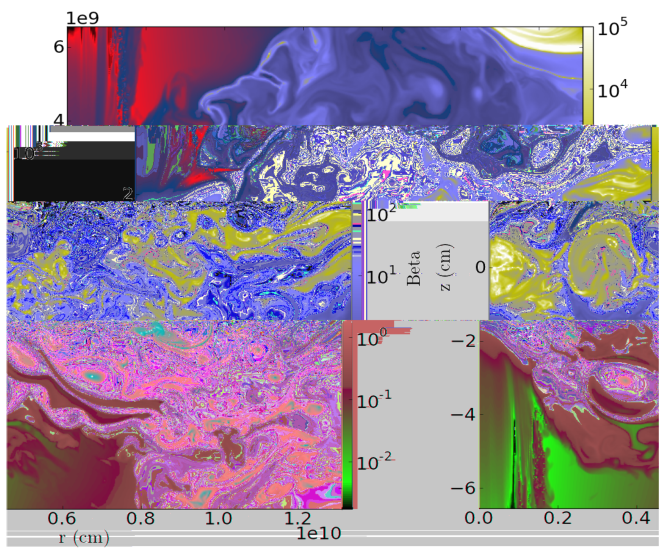
\includegraphics[width=\textwidth]{pictures/ji2_cropped.pdf}
\end{column}
\end{columns}
\begin{center}{ \tiny [White dwarf merger. Left: Magnetic field lines. Right: $\beta=$ Gas Pressure/Magnetic Pressure. Ji et al; 2013]}\end{center}
}

%%% Local Variables:
%%% mode: latex
%%% TeX-master: "main"
%%% End:
